% \begin{figure}[h!]
%     \centering

%     % =======================
%     % Top row: diagram + single example column
%     % =======================
%     \begin{minipage}{0.95\linewidth}
%         \centering
%         % Combined diagram and example
%         \begin{minipage}{0.5\linewidth}
%             \centering
%             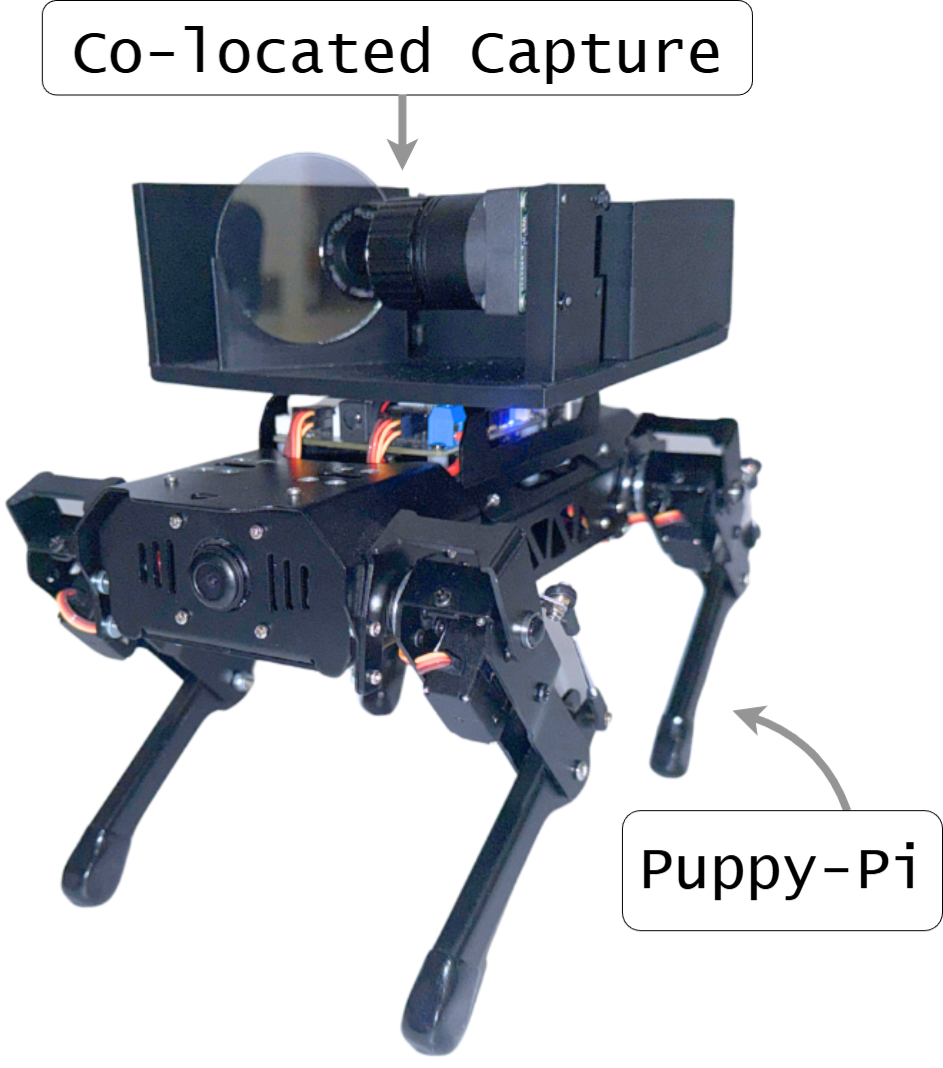
\includegraphics[width=\linewidth]{Figures/puppy-pi.drawio.png}
%         \end{minipage}%
%         \hspace{1mm}
%         \begin{minipage}{0.25\linewidth}
%             \centering
%             % Example column: Input / Prediction / Ground Truth
%             % Row 1 — Input
%             \begin{minipage}{0.2\linewidth}
%                 \centering
%                 \rotatebox{90}{\small Input}
%             \end{minipage}%
%             \begin{minipage}{0.75\linewidth}
%                 \centering
%                 
\includegraphics[width=\textwidth]{puppy-pi/rs/frame55.png}
%             \end{minipage}

%             \vspace{1mm}

%             % Row 2 — Prediction
%             \begin{minipage}{0.2\linewidth}
%                 \centering
%                 \rotatebox{90}{\small Prediction}
%             \end{minipage}%
%             \begin{minipage}{0.75\linewidth}
%                 \centering
%                 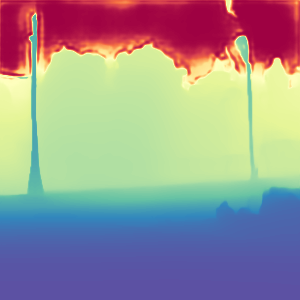
\includegraphics[width=\textwidth]{puppy-pi/depth/rs/frame55_pred.png}
%             \end{minipage}

%             \vspace{1mm}

%             % Row 3 — Ground Truth
%             \begin{minipage}{0.2\linewidth}
%                 \centering
%                 \rotatebox{90}{\small Ground Truth}
%             \end{minipage}%
%             \begin{minipage}{0.75\linewidth}
%                 \centering
%                 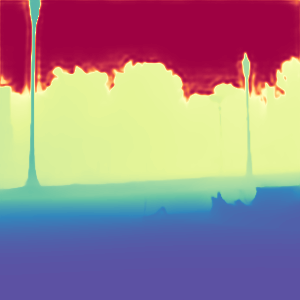
\includegraphics[width=\textwidth]{puppy-pi/depth/gs/frame55.png}
%             \end{minipage}
%         \end{minipage}
%     \end{minipage}

%     \vspace{2mm}

%     % =======================
%     % Bottom: Table
%     % =======================
%     \begin{minipage}{0.65\linewidth}
%         \centering
%         \begin{tabular}{lcc}
%             \toprule
%             Method & absRel $\downarrow$ & $\delta 1 \uparrow$ \\
%             \midrule
%             Raw RS Image & 0.1119 & 0.8958 \\
%             Our Algorithm & \textbf{0.0963} & \textbf{0.9033} \\
%             \bottomrule
%         \end{tabular}
%     \end{minipage}

%     \caption{Left: schematic illustration of the RS effect on the Puppy-Pi. Right: input, prediction, and ground truth for a single frame. Bottom: dataset-averaged depth metrics comparing raw RS input and corrected output. 
%     %\JI{What does this image/result mean...please revise @Vaishnav }
%     }
%     \label{fig:puppy}
% \end{figure}

\begin{figure}[t]
\centering
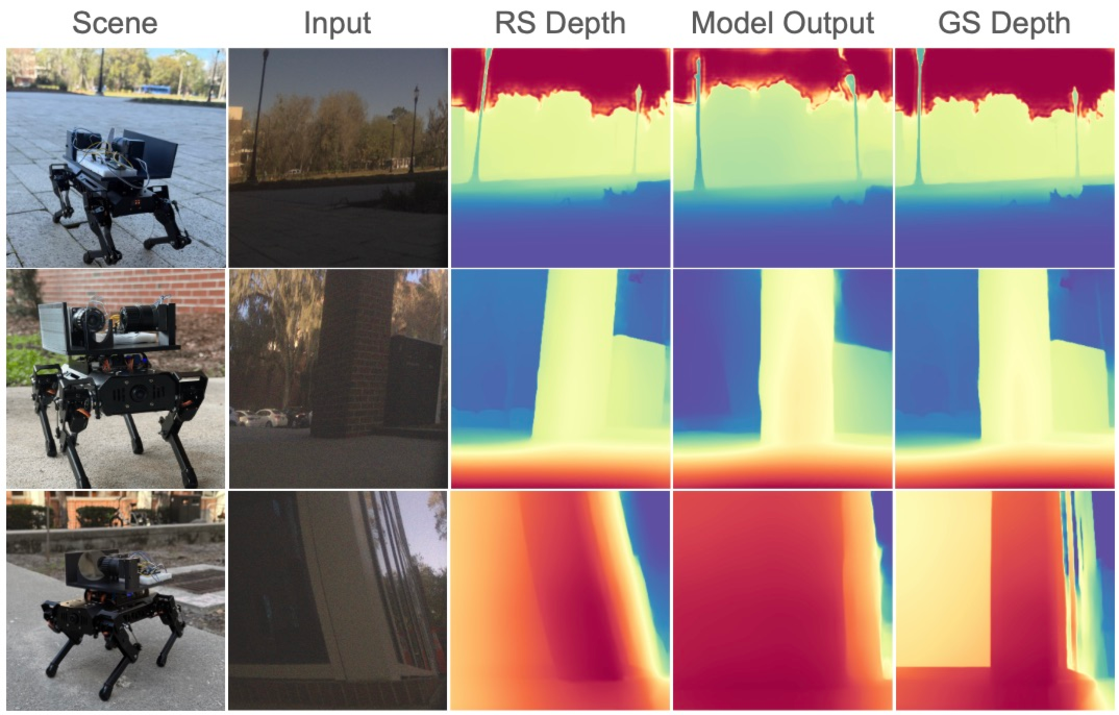
\includegraphics[width=0.49\textwidth]{Figures/puppy_pi_exp_short.pdf}
\caption{Visualizations of our model for RS distortions in legged robots. The qualitative results demonstrate effective rectification of rolling shutter artifacts in legged robotic scenarios.}
\label{Fig:puppy_pi_qual}
\vspace{-3mm}
\end{figure}